\documentclass[10pt,a4paper]{report}
\usepackage[a4paper,left=25mm,right=25mm,top=25mm,bottom=20mm]{geometry}
\usepackage{amsfonts}
\usepackage{graphicx}
\graphicspath{{./images/}}
\usepackage{csquotes}
\usepackage{hyperref}
\usepackage{listings}

\title{\huge{\textbf{Data Mining report}}}
\author{Funaioli Francesca\\
Karoui Hamza\\
Francesco Mitola\\
Vezzuto Samuele}

\begin{document}

\maketitle
\tableofcontents

\chapter{Data Understanding}

The data understanding phase aims to prepare data for the following data mining tasks and to gain informations on the general properties of our data.
We started by importing the three csv files, \texttt{incidents.csv}, \texttt{povertyByStateYear.csv} and \texttt{year\_state\_district\_house.csv}.
We did some preliminary checks, for example we looked for attributes containing null values, and then we started analysing each column of each dataset.

\subsection{Incidents}

\subsubsection{Date}

We converted each \textit{date} value to a datetime object: there where no null values or NaT values.
We then plotted the distribution of the dates over the years: we noticed that the dates ranged from year 2013 to year 2018 and from year 2028 to year 2030.
Year 2013 only contains 253 incidents so we consider removing these few rows; we also decided to delete incidents recorded in years from 2028 to 2030, because they are to happen after the date the dataset was provided.

\subsubsection{State}

The \textit{state} attribute contains no null values and it has 51 unique values: the 50 states of the United States and the District of Columbia.

\subsubsection{City or county}

The \textit{city\_or\_county} attribute has no null values; we noticed it contains additional informations about the suburb or the neighborhood in brackets, e.g. ``Minneapolis (Brooklyn Center)".
We consider removing this informations in the following phases.

\subsubsection{Address}

The \textit{address} attribute contains some null values, but we believe it does not hold any statistical value, given that a more specific information about the exact location of the incident is found by using the geographical coordinates.

\subsubsection{Latitude and longitude}

The \textit{latitude} and \textit{longitude} attributes contain some null values.
We also noticed some outliers by drawing empirical box boundaries of the United States: there are some incidents recorded outside of the U.S. that we will remove in the next phase.

\subsubsection{Congressional, State House and State Senate district}

These attributes contain some null values.
We also noticed that most of the incidents happened in the state of Illinois, by plotting the top 10 incidents for each of these attributes.

\subsubsection{Age and gender attributes}

The \textit{participant\_age1} attribute contains some outliers wrt the corresponding value reported in the \textit{participant\_age\_group1}.
There also some outliers, e.g. maximum value of \textit{participant\_age1} is 311.
We noticed that most of the participants are adult males.
The attributes \textit{participant\_age1}, \textit{min\_age\_participants}, \textit{max\_age\_participants} and \textit{avg\_age\_participants} all have similar distributions.
The attributes \textit{n\_participants\_child}, \textit{n\_participants\_teen} and \textit{n\_participants\_adult} all present the same issues: they all contain some outliers given by non-numerical strings, very large numbers or negative numbers.

\subsubsection{Number of involved people}

The majority of the incidents only involve between 0 and 5 people, with almost no killed, injured, unharmed or arrested people.

\subsubsection{Notes and incident characteristics}

We consider these attributes to hold no statistical value.

\subsection{Poverty by state}

The \textit{state} attribute contains 52 unique values: 51 of them are the same as the states in the incidents dataset, the remaining one is labeled ``United States" and contains the average of the whole country.
We consider using the average to possibly fill the missing values in the following phase.

There are no \textit{povertyPercentage} values for the year 2012, but we are only interested in relating this information to the incidents dataset, which only contains relevant incidents in the range of years 2013-2018.

\subsection{Year state district house}

This dataset contains no null values.
We will only consider data in the range of years 2013-2018 for integrating this data with the incidents dataset.

\section{Data integration}

We created an additional column called \textit{total\_votes\_for\_state} in the year-state-house-district dataset; this column contains the total number of votes for each state and for each year.
We merged the incidents dataset with the poverty dataset using the attributes \textit{state} and \textit{year}.
We then merged the resulting dataset with the remaining one using the attributes \textit{state}, \textit{year} and \textit{congressional\_district}.

\chapter{Data Preparation}

The data preparation phase uses the information gained in the previous phase to select records, manage outliers and missing values and improve data quality.
We started by changing the data types of the attributes as shown in Table \ref{table01}.

\begin{table}
	\centering
	\begin{small}
	\begin{tabular}{|l|l|l|p{7cm}|}
		\hline
		\textbf{Feature Name} & \textbf{Initial Type} & \textbf{Cast Type} & \textbf{Description}\\
		\hline
		date & object & Datetime64 & date of incident occurrence\\
		\hline
		state & object & String & state where incident took place\\
		\hline
		city\_or\_county & object & String & city or county where incident took place\\
		\hline
		address & object & String & address where incident took place\\
		\hline
		latitude & float64 & float64 & latitude of the incident\\
		\hline
		longitude & float64 & float64 & longitude of the incident\\
		\hline
		congressional\_district & int64 & Int64 & congressional district where the incident took place\\
		\hline
		state\_house\_district & int64 & Int64 & state house district\\
		\hline
		state\_senate\_district & float64 & Int64 & state senate district where the incident took place\\
		\hline
		participant\_age1 & float64 & Int64 & exact age of one (randomly chosen) participant in the incident\\
		\hline
		participant\_age\_group1 & object & String & exact age group of one (randomly chosen) participant in the incident\\
		\hline
		participant\_gender1 & object & String & exact gender of one (randomly chosen) participant in the incident\\
		\hline
		min\_age\_participants & object & Int64 & minimum age of the participants in the incident\\
		\hline
		avg\_age\_participants & object & float64 & average age of the participants in the incident\\
		\hline
		max\_age\_participants & object & Int64 & maximum age of the participants in the incident\\
		\hline
		n\_participants\_child & object & Int64 & number of child participants 0-11\\
		\hline
		n\_participants\_teen & object & Int64 & number of teen participants 12-17\\
		\hline
		n\_participants\_adult & object & Int64 & number of adult participants (18 +)\\
		\hline
		n\_males & float64 & Int64 & number of males participants\\
		\hline
		n\_females & float64 & Int64 & number of females participants\\
		\hline
		n\_killed & int64 & Int64 & number of people killed\\
		\hline
		n\_injured & int64 & Int64 & number of people injured\\
		\hline
		n\_arrested & float64 & Int64 & number of arrested participants\\
		\hline
		n\_unharmed & float64 & Int64 & number of unharmed participants\\
		\hline
		n\_participants & float64 & Int64 & number of participants in the incident\\
		\hline
		notes & object & String & additional notes about the incident\\
		\hline
		incident\_characteristics1 & object & String & incident characteristics\\
		\hline
		incident\_characteristics2 & object & String & incident characteristics\\
		\hline
		year & int64 & Int64 & \\
		\hline
		povertyPercentage & float64 & float64 & poverty percentage for the corresponding state and year\\
		\hline
		party & object & String & winning party for the corresponding congressional\_district in the state, in the corresponding year\\
		\hline
		candidateVotes & int64 & Int64 & number of votes obtained by the winning party in the corresponding election\\
		\hline
		totalVotes & int64 & Int64 & total number of votes for the corresponding election\\
		\hline
		total\_votes\_for\_state & int64 & Int64 & total number of votes for each year and for each state\\
		\hline
	\end{tabular}
	\end{small}
	\caption{Features of the merged dataset}
	\label{table01}
\end{table}

We then removed negative values by setting them to NaN.

\subsubsection{Age attributes}

For the attributes \textit{participant\_age1}, \textit{min\_age\_participants}, \textit{max\_age\_participants} and \textit{avg\_age\_participants}, we considered values $\ge 120$ as outliers and we set them to NaN.
These three attributes seemed to be very correlated, so we consider deleting the columns \textit{min\_age\_participants} and \textit{max\_age\_participants} and only keeping \textit{avg\_age\_participants}.

\subsubsection{Date}

We considered all dates after 2023-10-01 (the date we received the dataset) to be outliers, in particular errors in the data.
We dropped all records related to year 2013, as the year was under-represented (only 242 records).

\subsubsection{Geographical attributes}

The records with coordinates outside U.S. (other that null values) were automatically deleted after the data integration.
We consider the triple \textit{$<$date,latitude,longitude$>$} to be a key identifying an incident: we assume that there are no incidents happening on the same day in the exact same geographic coordinates.
Hence, we decided to eliminate the records in which these 3 values are duplicate.

For the rows in which \textit{latitude} and \textit{longitude} are NaN, we filled the missing values using the mean computed for the respective \textit{state} and \textit{city\_or\_county}.

We decided to drop the columns \textit{state\_house\_district} and \textit{state\_senate\_district}, given that they represent further subdivisions of the US territory that are not pertinent to our analysis.
In fact, we are only interested in the \textit{congressional\_district}, because the electoral information has the same granularity.

\subsubsection{Number of participants' attributes}

We checked whether the number of killed, injured, arrested and unharmed people exceeded the total number of participants in that incident.
Since, \textit{n\_arrested} and \textit{n\_killed} were the only two attributes with null values, we set them to 0 in case \textit{n\_participants} was 0; we filled the remaining null values using the mean.

We set to NaN the outliers found in \textit{n\_participants\_adult}, \textit{n\_participants\_teen} and \textit{n\_participants\_child} found during data understanding.
The outliers considered in this step were the values larger than the maximum values of \textit{n\_participants}.
We also set to zero the attributes \textit{n\_participants\_adult}, \textit{n\_participants\_teen}, \textit{n\_participants\_child}, \textit{n\_males} and \textit{n\_females} when \textit{n\_participants} is 0.
We replace the value in \textit{n\_participants} with the sum \textit{n\_males} + \textit{n\_females}, if this sum is equal to (\textit{n\_participants\_adult} + \textit{n\_participants\_teen} + \textit{n\_participants\_child}) and different from \textit{n\_participants}.
Viceversa, we set to NaN these attributes in the rows where the sums and/or \textit{n\_participants} are not equal.
We then substituted NaN values using the mean of each attribute and dropped the few rows for which we were not able to reconstruct the mean.

\subsubsection{Incident characteristics}

We dropped the column \textit{incident\_characteristics2} given that it has 40\% of null values and does not add meaningful details for our analysis.

\section{Correlation analysis}

We plotted the correlation matrix (Figure \ref{corr_matrix}) only for the numerical attributes.
We noticed that age attributes are highly correlated: we decided to drop all of them\footnote{We dropped \textit{participant\_age1}, \textit{min\_age\_participants} and \textit{max\_age\_participants}.} except for \textit{avg\_age\_participants}, which is the most correlated to the other attributes and gives us more general informations about all the participants.
Given the fact that we dropped \textit{participant\_age1}, then the attributes \textit{participant\_gender1} and \textit{participant\_age\_group1} become useless, so we dropped them.
To fill NaN values in \textit{avg\_age\_participants} we used the mean of each grouping on \textit{n\_participants}.

\begin{figure}[h]
	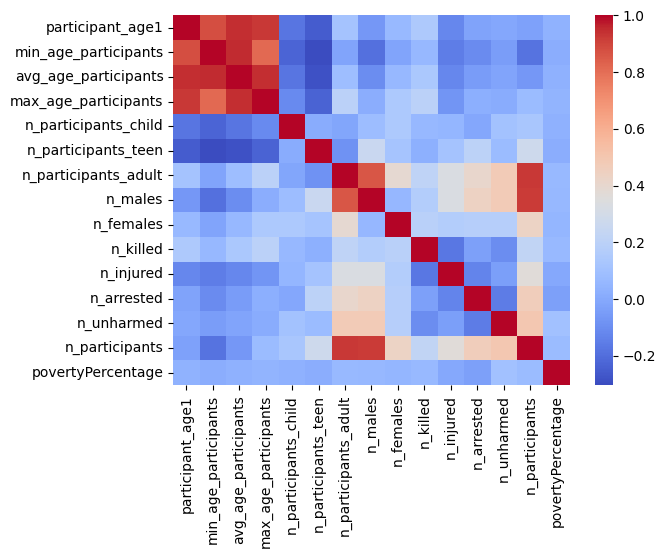
\includegraphics[width=0.8\textwidth]{corr_matrix}
	\centering
	\caption{Correlation matrix plotted of the numerical attributes}
	\label{corr_matrix}
\end{figure}

\section{Definition of indicators}

We computed the following indicators:
\begin{itemize}
	\item \textit{males\_percentage\_per\_city} (\textit{females\_percentage\_per\_city}), the number of males (females) involved in an incident over the total number of males (females) involved in incidents in the same city over the same time period;
	\item \textit{killed\_percentage\_per\_district} (\textit{injured\_percentage\_per\_district}, \textit{arrested\_percentage\_per\_district}, \textit{unhar\-med\_percentage\_per\_district}), the number of killed (injured, arrested, unharmed) people in an incident over the total number of people killed (injured, arrested, unharmed) in incidents in that same congressional district over the same time period;
	\item \textit{killed\_percentage\_per\_incident}, the number of killed people in each incident over the total number of participants in that same incident;
	\item \textit{unharmed\_percentage}, the number of unharmed people in the incident over the average of unharmed people in all the incidents in the same time period;
	\item \textit{arrest\_percentage}, the number of arrested people over the total number of participants in each incident;
	\item \textit{killed\_rate\_per\_state} (\textit{injured\_rate\_per\_state}, \textit{arrested\_rate\_per\_state}, \textit{unharmed\_rate\_per\_state}), the total number of people killed (injured, arrested, unharmed) per date and state over the total number of people killed (injured, arrested, unharmed) in that same date;
	\item \textit{age\_entropy\_per\_state}, the entropy of the \textit{avg\_age\_participants} grouped for date and state;
	\item \textit{winning\_party\_percentage}, the number of votes of the winning candidate over the total number of votes for that election.
\end{itemize}

We then plotted the correlation matrix (Figure \ref{corr_matrix_indicators}) for the indicators defined above.

\begin{figure}[h]
	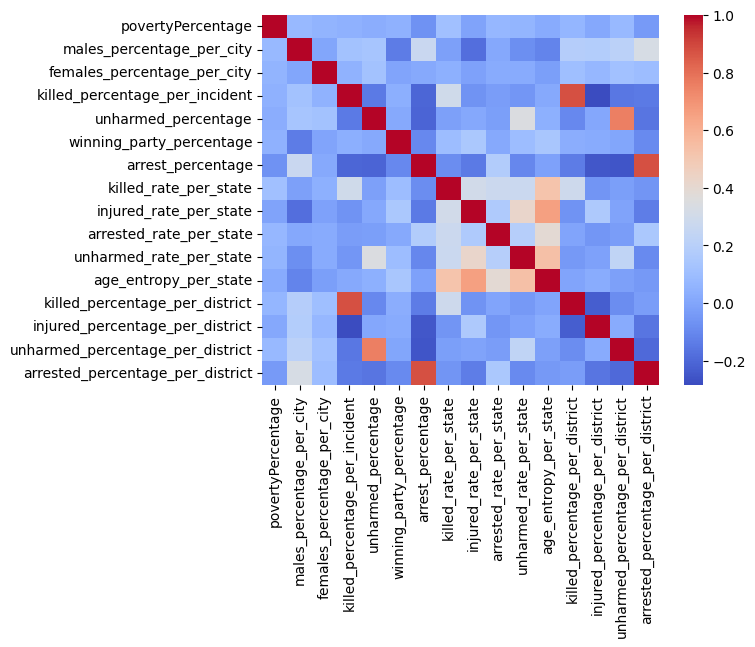
\includegraphics[width=0.8\textwidth]{corr_matrix_indicators}
	\centering
	\caption{Correlation matrix plotted of the newly created indicators}
	\label{corr_matrix_indicators}
\end{figure}

We also decided to drop the columns \textit{year} (just a result of data integration), \textit{address} and \textit{notes}.

\chapter{Clustering}

In order to prepare data for applying the clustering algorithms, we did some steps of preprocessing.
First of all we added a binary column \textit{involve\_killing} that has value 0 nobody was killed in the incident, and it has value 1 if there was at least a person killed in the incident.
We applied a normalization to numerical values.
The we computed the PCA with 2 components and got the visualization showed in Figure \ref{pca}.

\begin{figure}[h]
	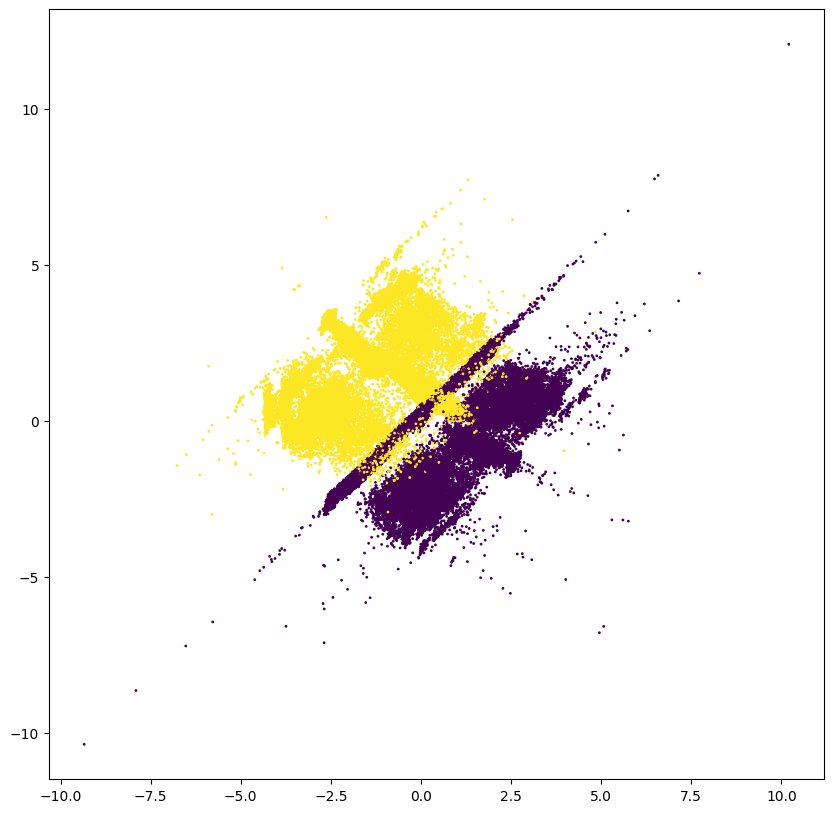
\includegraphics[width=0.8\textwidth]{pca}
	\centering
	\caption{Principal component analysis, computed on 2 components.
	The color of the points corresponds to the value of \textit{involve\_killed}.}
	\label{pca}
\end{figure}

\section{K-Means}

\subsection{X-Means}

\section{Hierarchical clustering}

\section{Dbscan clustering}

\end{document}
